
\documentclass[12pt]{article}
\usepackage[paper=letterpaper,margin=2cm]{geometry}

\usepackage{amsmath}
\usepackage{amsthm} %needed for the proofs 
\usepackage{amssymb}
\usepackage{titling}
\usepackage{thmtools}
\usepackage{mathptmx} %font
\usepackage{verbatim} % for comments
\usepackage{mdframed}
\usepackage[linesnumbered,ruled,vlined]{algorithm2e}
\usepackage{lipsum}

\usepackage[T1]{fontenc} %header
\usepackage[utf8]{inputenc}%header
\usepackage{geometry} %header
\usepackage{fancyhdr}%header

%images
\usepackage{graphicx}
\graphicspath{ {./images/} }
% to include an image, do: 
%    \begin{center}
%    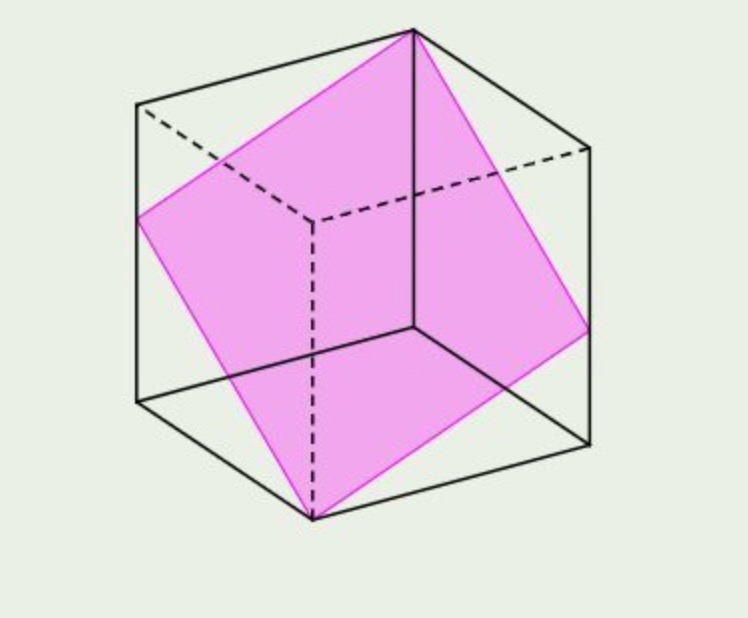
\includegraphics[scale=0.20]{graph.jpg}
%    \end{center}
% OR: 
%\begin{figure}
%    \centering
%    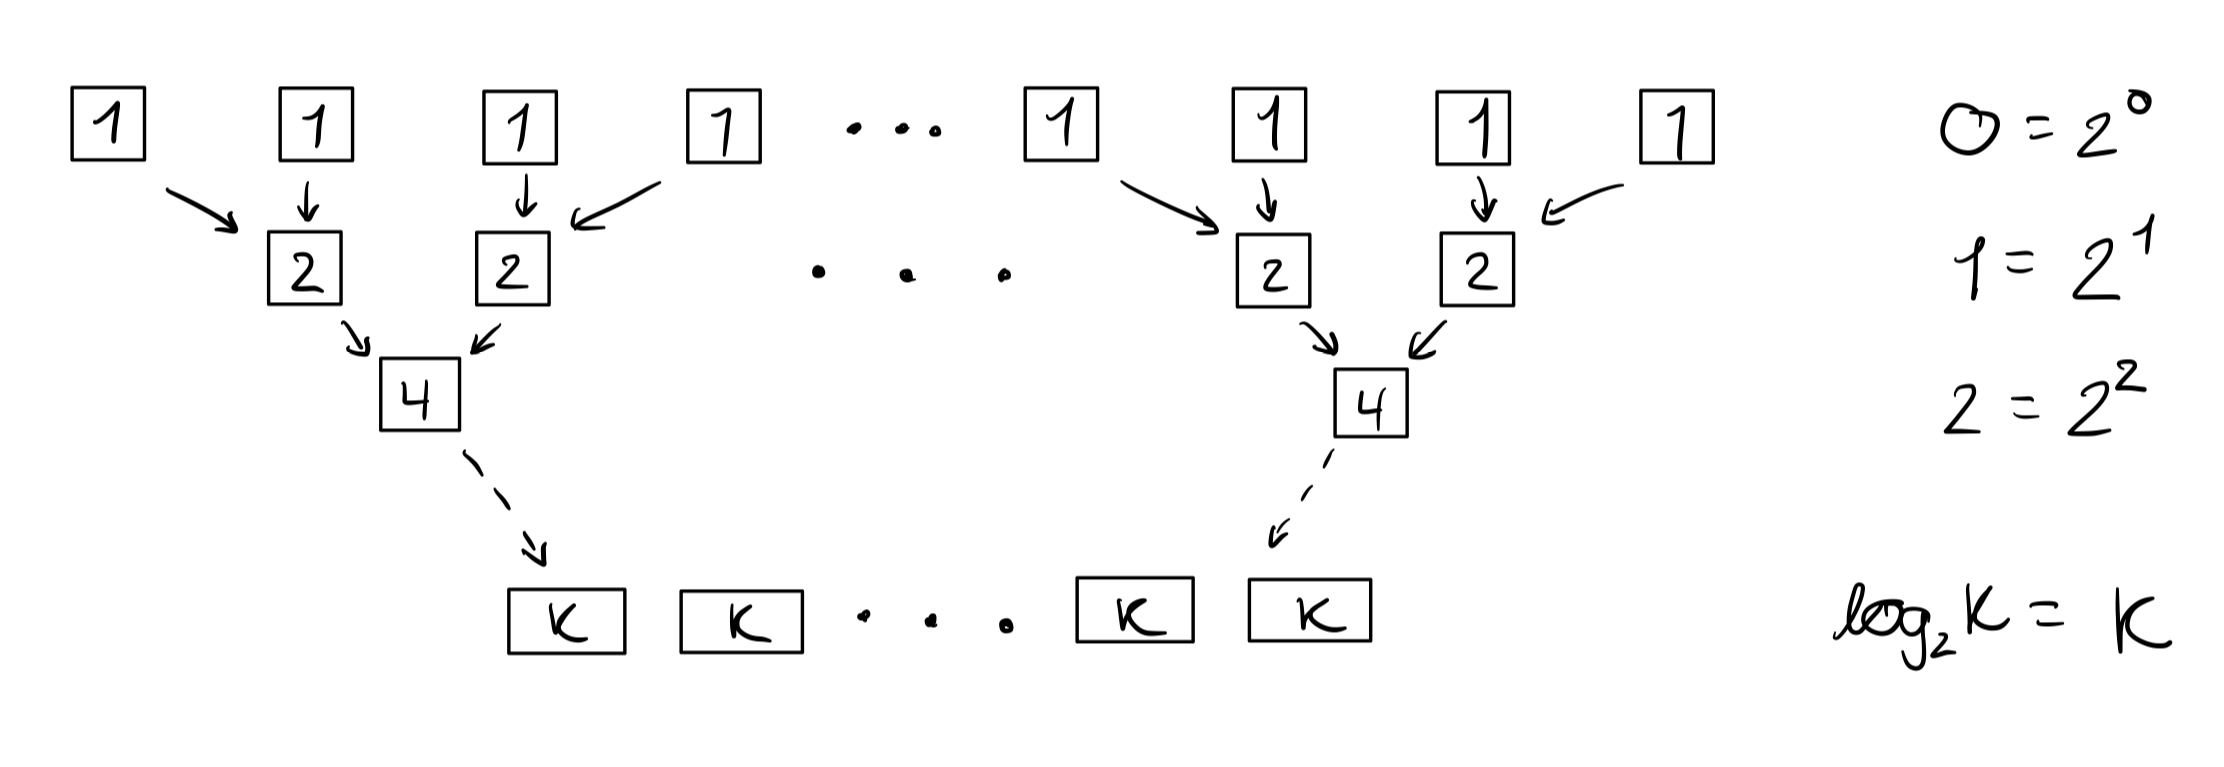
\includegraphics[scale=0.20]{IMG_1052.jpg}
%    \caption{Your caption text here.}
%\end{figure}
\renewcommand{\headrulewidth}{.4mm} % header line width

\pagestyle{fancy}
\fancyhf{}
\fancyhfoffset[L]{1cm} % left extra length
\fancyhfoffset[R]{1cm} % right extra length
\rhead{\today}
\lhead{\it Alexandre St-Aubin \& Jonathan Campana}
\rfoot{}

%macros for recursive functions
\newcommand{\forcond}{$i=0$ \KwTo $n$}
\SetKwFunction{FRecurs}{MaxSubArray}%
\SetKwProg{Fn}{Function }{\string:}{}
\SetKwData{Left}{left}\SetKwData{This}{this}\SetKwData{Up}{up}
\SetKwFunction{Union}{Union}\SetKwFunction{FindCompress}{FindCompress}
\SetKwInOut{Input}{input}\SetKwInOut{Output}{output}
%For plots
\usepackage{pgfplots}
\pgfplotsset{compat = newest}

\newtheorem{theorem}{Theorem}
\declaretheoremstyle{lemma}
\declaretheorem[style=lemma, name=Lemma]{lemma}

\theoremstyle{definition}
\newtheorem{definition}{Definition}

\declaretheoremstyle{example}
\declaretheorem[style=example, name=Example]{example}

\theoremstyle{remark}
\newtheorem*{remark}{Remark}

\declaretheoremstyle{proposition}
\declaretheorem[style=proposition, name=Proposition]{proposition}

\declaretheorem[name=Note]{note}
\declaretheoremstyle{note}

\setlength\parindent{24pt}%set paragraph indent

\newenvironment{ftheo}
  {\begin{mdframed}\begin{theorem}}
  {\end{theorem}\end{mdframed}}

\newcommand\sol{%
  \\ 
  \\
  \textit{Solution:}\\%
}

\setlength{\droptitle}{-6em}

\title{\textsc{Assignment 2 -- Comp 252}}  
\author{Alexandre St-Aubin \& Jonathan Campana}
\date{\today}

\begin{document}
\maketitle 
\begin{enumerate}
  \item \textsc{Algorithm Design.}
You are given $n$ vectors $x_1,... , x_n$ in $\mathbb{Z}^n$. Design an efficient algorithm in the ram model for computing for each $x_i$ one of its nearest
neighbors among the other points, using the standard Euclidean metric to measure distances. You can’t
use real numbers, and operations like square root are not available. Nevertheless, show how this can be
done in $o(n^3)$ worst-case time.
\sol   
   We first note that minimizing the Euclidean distance between 2 vectors of length $n$ is equivalent to minimizing the sum of squared differences between each individual components. The reason for this is that the square root is a monotone increasing function. Let $x_i = (x_{i,1}, ..., x_{i,n}), \; x_j = (x_{j,1}, ..., x_{j,n})$ both in $\mathbb{Z}^n$, and define 
  \begin{equation}d_2^2(x_i, x_j) := \sum_{k=1}^n (x_{i,k} -x_{j,k})^2 = \sum_{k=1}^n(x_{i,k}x_{i,k} - 2 x_{i,k} x_{j,k} + x_{j,k}x_{j,k}) = \langle x_i, x_i  \rangle + 2\langle x_i, x_j  \rangle  + \langle x_j, x_j  \rangle \end{equation}
  It is obvious that $d_2^2 \sim O(n)$ in the \textsc{ram} model , and that no real numbers, nor square roots were used to compute it. Now, we notice that $\frac{n(n-1)}{2}$ distances need to be computed, and in view of dynamic programming, we find a way to compute everything at once in order to reduce the complexity that would occur if we were to get each $d_2^2$ individually, namely, $O(n^3)$. Construct the following matrix, 

  $$ X = \begin{pmatrix}
    x_{1,1} & x_{1,2} & x_{1,3} & \hdots & x_{1,n} \\ 
 x_{2,1} & x_{2,2} & x_{2,3} & \hdots & x_{2,n} \\
 x_{3,1} & x_{3,2} & x_{3,3} & \hdots & x_{3,n}\\ 
    \vdots & \vdots & \vdots & \ddots & \vdots \\ 
     x_{n,1} & x_{n,2} & x_{n,3} & \hdots & x_{n,n}
  \end{pmatrix} $$
  Then, 
  $$X \cdot X^T = \begin{pmatrix}
    \sum_{k = 1}^n x_{1,k}x_{1,k} & \sum_{k = 1}^n x_{1,k}x_{2,k} & \hdots  & \sum_{k = 1}^n x_{1,k}x_{n,k} \\ 
    \sum_{k = 1}^n x_{2,k}x_{1,k} & \sum_{k = 1}^n x_{2,k}x_{2,k} & \hdots  & \sum_{k = 1}^n x_{2,k}x_{n,k} \\ 
\vdots & \vdots & \ddots & \vdots \\ 
    \sum_{k = 1}^n x_{n,k}x_{1,k} & \sum_{k = 1}^n x_{n,k}x_{2,k} & \hdots  & \sum_{k = 1}^n x_{n,k}x_{n,k}
  \end{pmatrix} = \begin{pmatrix}
    \langle x_1, x_1  \rangle &\langle x_1, x_2  \rangle & \hdots & \langle x_1, x_n  \rangle \\ 
\langle x_2, x_1  \rangle &\langle x_2, x_2  \rangle & \hdots & \langle x_2, x_n  \rangle \\ 
\vdots & \vdots & \ddots & \vdots \\ 

\langle x_n, x_1  \rangle &\langle x_n, x_2  \rangle & \hdots & \langle x_n, x_n  \rangle  

  \end{pmatrix}  $$

where the entries of $X \cdot {X^T}$ are exactly the dot products needed in (1). 
Therefore, by employing \textsc{Strassen's} algorithm, we can efficiently compute the product $X \cdot {X^T}$ with a time complexity of $O(n^{2.807})$. Subsequently, each of the $\frac{n(n-1)}{2} $ distances can be computed in $O(n^2)$ time, as computing one distance will take constant time by accessing the dot products in the matrix previously computed. Simultaneously, these distances can be added to an ordered list (corresponding to each individual vector) in constant time. Upon completion of this process, we will have the closest vector to any given vector readily accessible. The algorithm outlined above has a complexity of $O(n^{2.807})$, demonstrating that it can be accomplished in worst-case time less than $o(n^3)$.

  \newpage 
  \item \textsc{Dynamic programming: computing the optimal star.}  
  \begin{algorithm}
    \caption{Algorithm to compute the optimal star.}
    \SetKwInput{KwOut}{Output}
    \KwIn{A matrix $D[i,j]$ of pairwise distances between cities $1 \leq i,j \leq n$. }
    \KwOut{The cost of the optimal star that links the given cities.}
    \BlankLine
    \tcp{initialize M[v, S] for sets of size 1}
    \For{all $i\in [1,n]$}{
      \For{all $j\neq i $}{
      $M[i, \{j\}] \leftarrow D[i,j] $ ;  
      }
    }\BlankLine
\tcp{loop through each central city}
    \For{all $v\in [1,n]$}{
    \tcp{loop through each subset size}
       \For{all $k\in [1, n-1]$ }{
       \tcp{loop through each subset of size k excluding the central city}
          \For{all $S$ with $|S| = k,\; S \subseteq \{1, ..., n\}\setminus\{v\}$ }{
              $M[v,S] \leftarrow \min_{l\in S} \left\{ M[v, S\setminus \{l\}] + \min\{d(l, x) \; : \; x = v 
              \text{ or } \deg(x) = 1\}\right\}$; 
          } 
       }
    }\BlankLine
    
    \Return $\min_{v \in [1,n]} \left\{M[v, S] : |S| = n \right\}$


  \end{algorithm}

  \begin{remark} 
    The above is heavily inspired from the \textit{Held–Karp algorithm}, which was presented in class. 
  \end{remark}
  \textbf{Analysis of the algorithm}

\hspace{24pt} Allow $\Omega$ to represent the set of all vertices (cities). The outer loop iterates through each potential central vertex $v$ of the star, while the subsequent loops systematically explore subsets of $\Omega\setminus {v}$ in a bottom-up fashion. Starting with subsets of size $1$ (i.e., $S = {s}$), we know $M[v,S] = d(v, s)$. We then progress through sets of increasing size, using our knowledge from preceding, smaller sets to obtain an optimal set length, until we reach $M[v, \Omega\setminus v]$,  thereby identifying the optimal star configuration with the central vertex $v$. 

\hspace{24pt} Let's delve into the time complexity analysis. Line 4 executes $n$ times. Lines 5 and 6 represent all possible subsets of a set with $n-1$ vertices, resulting in $2^{n-1}$ iterations. We can safely assume line 7 to be $O(n)$. Combining these components, the overall time complexity is given as $O(n^2 \cdot 2^n)$. We note that lines 1 \& 8 run in $O(n)$ time, so they play no significant role in the overall time complexity of the algorithm. 

\newpage 
  \item \textsc{Induction.} We are given the recurrence 
  $$T_n = 2 T_{\frac{n}{a}} + 7 T_{\frac{n}{a^2}} + 1,$$
  where $a \geq 2$ is a given integer, and $n$ is restricted to be a power of $a$. We also know that $T_1 = T_a = 1$.\newline
  \begin{enumerate}
    \item[\it (a)] $T_n = \Omega(n^c)$ for some constant $c.$
\begin{proof} For the base case, let $n = a^2$, then, 
  $$T_{a^2} = 2 T_a + 7T_1 + 1 = 2 + 7  + 1 = \Omega(1) = \Omega(n^0), $$
  Now, assume $T_{a^k} = \Omega ((a^k)^c)$, for any $2\leq k < n$, then we have 
  \begin{equation*}
    \begin{split}
      T_{a^n} &= 2 T_{a^{n-1}} + 7T_{a^{n-2}} + 1\\ 
      &\leq 2 ((a^{n-1})^c) + 7((a^{n-2})^c) + 1 \quad [\text{by I.H.}]\\ 
      & \leq 9 (a^{n-1})^c \\
      & = \frac{9}{a^c} \left( a^n\right)^c \\ 
    \end{split}
  \end{equation*}
  Where $\frac{9}{a^c} $ is a constant so we conclude that $T_{a^n} = \Omega ((a^n)^c)$. Remains to find the largest such $c.$
\end{proof}
  \end{enumerate}
  \newpage
  \item  \textsc{Sorting with Duplicates.} \begin{enumerate}
    \item[\it (i)] Give a divide-and-conquer algorithm that sorts $n$ numbers with $1\leq k\leq n$ uniques. This can be done in time $O(n \log_2(k + 1))$ with a ternary comparison oracle. 
    
    \textit{See Algorithm 2 on next page.}
   \item[\it (ii)] Prove the complexity claim.
   \begin{proof} 
     For the sake of simplicity, we assume that $k = 2^i$ for some $i \in \mathbb{N}$. To prove that the complexity of our algorithm is $O(n \log(k+1)),$ we count the number of times that it uses the ternary oracle (number of comparisons made), as the rest costs 0, by the oracle model of complexity. We notice that the comparisons occur only at the \textit{merge} step of the algorithm, so we'll start counting at the first merge, namely when we have $n$ subarrays of size 1. We assume the worst case, i.e. that no duplicates are found in the merges until level $\log_2k$ is reached (see Figure \ref{fig1}). When this level is reached, we have $\frac{n}{k}$ sets of length at most $k$, and the next step will surely find duplicates, thereby reducing the running time compared to plain old merge sort. 
     

     \hspace{24pt} Let's count the number of comparison needed to get to level $\log_2k$ of the merging. In order to get one subarray of length $k$, $k$ subarrays of length 1 must be merged into 1. This process will take $\log_2 k$ merges, each one costing $\frac{(2^i-1)k}{2^i}$ comparisons, that is, 
     $$\sum^{\log_2 k}_{i=1} \frac{(2^i-1)k}{2^i} \leq \sum^{\log_2k}_{i=1} k = n \log_2 k \text{  comparisons.} $$
     And, since there are $\frac{n}{k}$ such subarrays, it follows that the complexity of the above process is $O(n \log_2 k).$ 
  

     \hspace{24pt} We now consider the second and last part of our computation. At this step, we have $\frac{n}{k}$ sets of size $k$. In the normal merge sort algorithm, the next step would generate half as many sets of double the size ($2k$). However, our algorithm combines duplicate terms into a single tuple element, and since there are only $k$ elements that are different in our set, $k$ is an upper bound for the size of a subarray. Hence, we instead obtain half the amount of sets, but still of size at most $k$. This is also true for all the following merges. 

    
     \hspace{24pt} Let's compute the time complexity of merging $\frac{n}{k}$ subarrays until we have 1 array of length $k.$ Well, it is clear that each merge will cost at most $k$ comparisons, as in the worst case, we are merging two arrays of length $k,$ which must therefore be identical, as they are ordered and contain the same k elements. Thus, the oracle will yield $k$ equalities, which suffices to merge the arrays. So, the total number of comparisons is given by 
     $$k \sum^{\log_2 \frac{n}{k}}_{i=0}  2^i = k (2^{\log_2 \frac{n}{k} }-1) = k \left( \frac{n}{k} -1 \right) = n-k  $$
     Combining both processes, it is easy to see that the total time complexity is 
     $$O(n-k + n \log_2 (k) ) = O(n \log_2 (k + 1)) $$
\begin{remark} 
  The reason why the complexity is $O(n\log_2(k+1))$, and not $O(n\log_2(k))$ is that in the case where $k = 1$, if we need the complexity to be $O(n \log_2 (1))$, not $O(0)$. 
\end{remark}
\begin{figure}
    \centering
    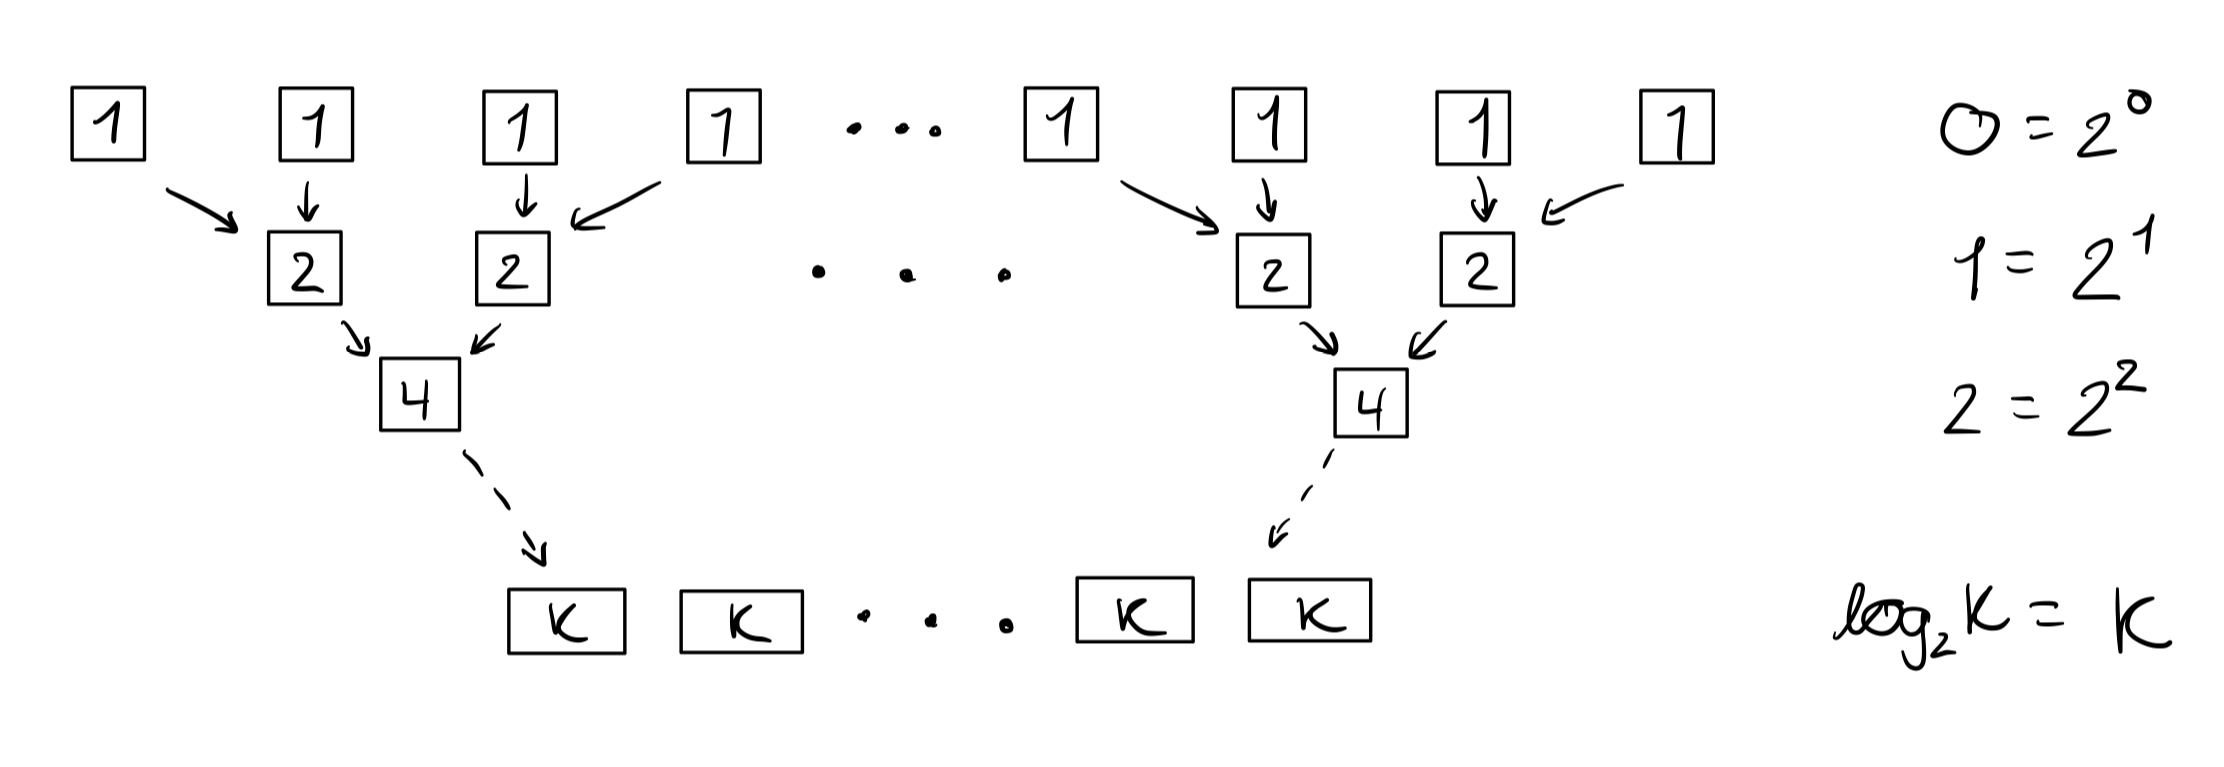
\includegraphics[scale=0.20]{IMG_1052.jpg}
    \caption{The merging of subarrays.}
    \label{fig1}
\end{figure}
   \end{proof}

  \begin{algorithm}
    \caption{DC algorithm to sort a list of $n$ elements with $1\leq k\leq n$ duplicates. }
    \SetKwFunction{ms}{MergeSort}
    \SetKwFunction{me}{Merge}
    \SetKwFunction{eq}{TernaryOracle}
    \SetKwArray{arr}{array}
    \SetKwArray{L}{Left}
    \SetKwArray{R}{Right}
    \SetKwData{mid}{mid}
    \SetKwInput{KwIn}{Input}
    \SetKwInput{KwOut}{Output}
    \KwIn{An arbitrary \arr of integers.}
    \KwOut{The sorted array.}
    \BlankLine
    \tcp{Initialize the array with Tuples }
    \For{$i = 0$ to $l(\arr)$ }{
    $\arr[i] \leftarrow$ new Tuple$(i, 1)$; \\ 
    }\BlankLine

    \tcp{ A function to compare tuples, each use costs 1. Anything else is free.}
    \Fn{\eq {tuple1, tuple2}}{
    \If{tuple1[0] = tuple2[0]}{
    \Return 0; 
    }\ElseIf{tuple1[0] < tuple2[0]}{\Return -1;}
    \Else{\Return 1;}
    }\BlankLine
    \Fn{\ms{\arr}}{
    \eIf{l(\arr) < 2}{\Return \arr;}{
\mid $\leftarrow \lfloor l(\arr)/2 \rfloor$; \\ 
    \Return \me(\ms(\arr[:\mid]), \ms (\arr[\mid :]));}
    }\BlankLine
    \Fn{\me{\L, \R}}{
    $i,j \leftarrow 0;$ \\ 
    \arr $\leftarrow $ new array; \\ 
    \While{$i \leq l(\L)\;\& \&\; j \leq l(\R)$}{
\Switch{$\eq{\L[i], \R[j]}$}{
\uCase{$0$}{
$\arr [i+ j] \leftarrow$ new Tuple$(\L[i][0], \L[i][1]+\R[i][1])$ ;\\ 
    $i ++, \; j ++ $;
}
\uCase{$1$}{
    $\arr [i+ j] \leftarrow \L[i]$ ;\\ 
    $i++;$
}
\uCase{$-1$}{ $\arr [i+ j] \leftarrow \R[j]$ ;\\ 
    $j++;$
}

    } \tcp{then add the rest of the array that we didn't reach the end of to the current array:}
    }$\arr \leftarrow \arr \& (i\leq l(\L))*\L[i: l(\L)] \& (j\leq l(\R))*\R[j: l(\R)]  $
}


  \end{algorithm}


  \end{enumerate}

\end{enumerate}
 
\end{document}
